The tests were conducted using 4 nodes connected to a gateway. The nodes were placed one on each shelf of the experimental rig in order to see how the height of the shelf affects vibrations, 
similar to a tall building. The nodes were securely mounted and calibrated until they were stable enough to not be affected by small vibrations which could corrupt the actual data. 
This would also apply to a real world scenario, where the nodes would need a sturdy mounting place to properly sense relevant vibrations in the structure of the building.

We have conducted 4 test runs by setting the supply voltage for the shake table's motors at different values. The shake table was powered on for 3 seconds during each test run. The first test is performed with a still table to verify just how sensitive the sensor nodes are. Then, we simulated 3 types of vibrations generated by different movements: small vibrations obtained by swaying the test table, medium vibrations obtained by shaking the test table and large vibrations obtained by 
violently shaking the test table.

We are interested in two specific results from this experiment. First, we want to see that the sensor readings are proportional to the type of vibration applied to 
the experimental rig. Second, we want to see how the sensor readings vary in relation to height. It is known that for tall objects such as buildings, the higher you 
go, the more intense the effects of vibrations become.

In figure \ref{fig:sensor-4} we see the accelerometer readings for the sensor placed on the lowest shelf (sensor ID 4) of the experimental rig taken during each test run. The
readings show that while the table is still, the sensor is stable and does not present any relevant activity. As we start increasing the intensity of the vibrations,
more and more spikes appear in the readings and they start reverting to normal as the vibrations stop. This shows that the Sparrow v4 sensors can reliably record 
the intensity of an event.

\begin{figure}[ht] \centering
  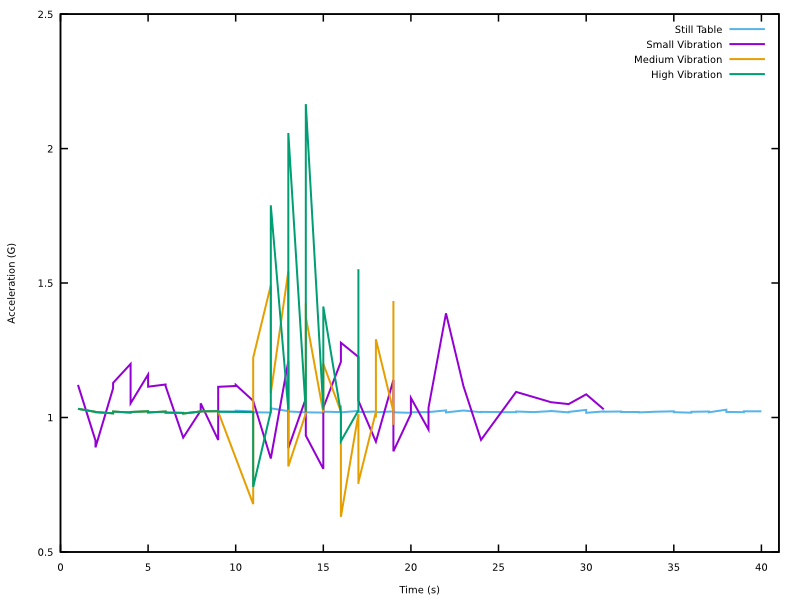
\includegraphics[width=0.5\textwidth]{img/sensor-4-data}
  \caption{Results for sensor 4 at different intensities}
  \label{fig:sensor-4}
\end{figure}

The other 3 graphs: \ref{fig:sensor-5}, \ref{fig:sensor-6}, \ref{fig:sensor-7} show the reading taken from the other sensors (IDs 7, 6 and 5). In the experimental setup, sensor ID 7 was placed above sensor ID 4, making it 
the second lowest. Then, sensor ID 6 was placed and the, at the highest level, sensor ID 5. The graphics show that the higher the sensor was placed, the interval between spikes near 2G increases and the 
amplitude of the readings also increases, sometimes going above 2G.

\begin{figure}[ht] \centering
  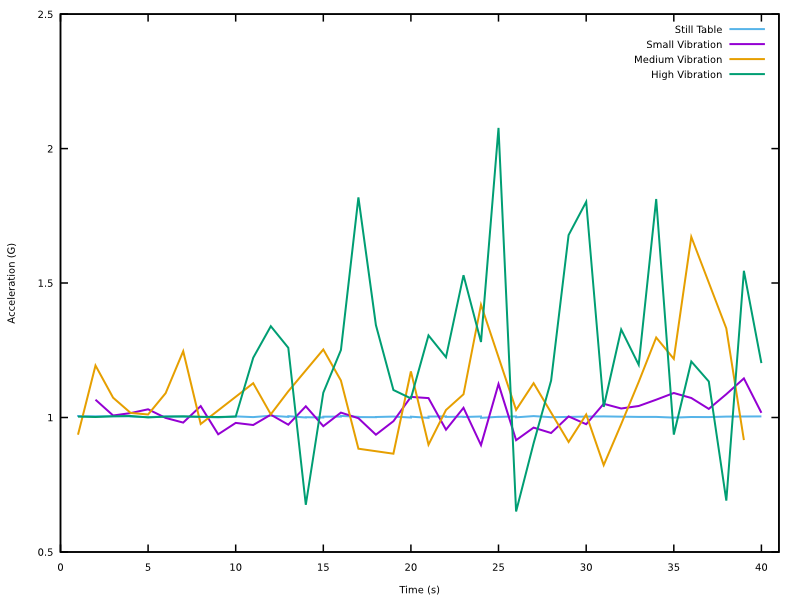
\includegraphics[width=0.5\textwidth]{img/sensor-7-data}
  \caption{Results for sensor 7 at different intensities}
  \label{fig:sensor-7}
\end{figure}

\begin{figure}[ht] \centering
  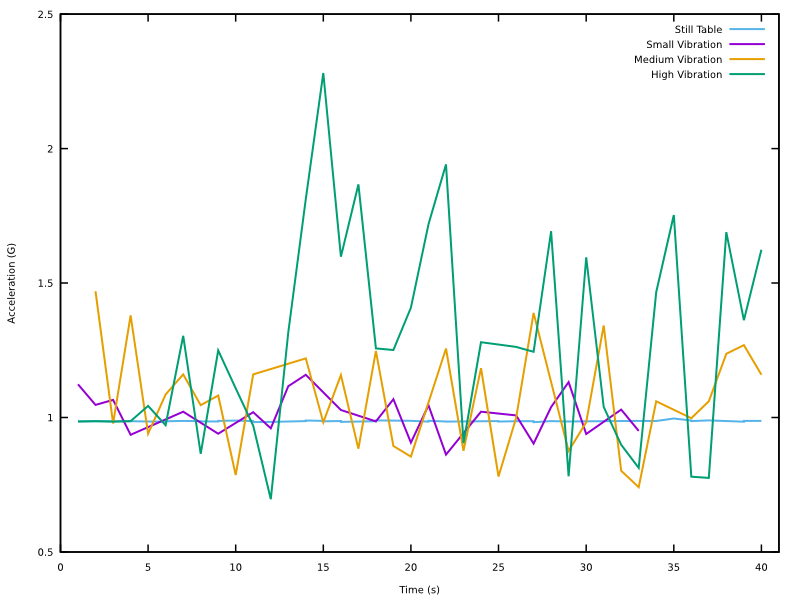
\includegraphics[width=0.5\textwidth]{img/sensor-6-data}
  \caption{Results for sensor 6 at different intensities}
  \label{fig:sensor-6}
\end{figure}

\begin{figure}[ht] \centering
  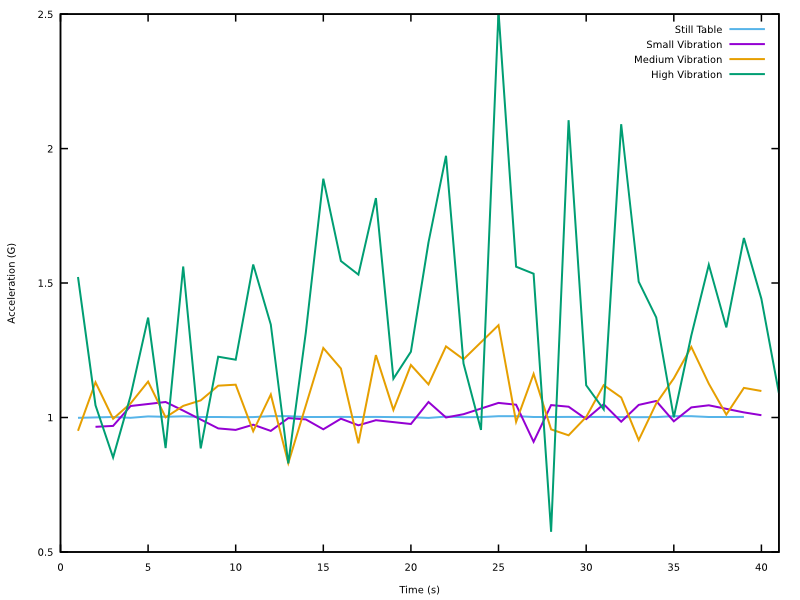
\includegraphics[width=0.5\textwidth]{img/sensor-5-data}
  \caption{Results for sensor 5 at different intensities}
  \label{fig:sensor-5}
\end{figure}

Another observation can be made regarding the calibration step. As it can be seen in~\ref{fig:sensor-6}, while the normal value for the other sensors is around 1G, sensor 6 is
slightly below this value. This happens because not all IMU modules are identical by fabrication, and it must be taken into account when interpreting the data. It also shows 
why the calibration step is important and necessary.

In figure \ref{fig:same-level} we see the accelerometer readings for all 4 sensors taken during the same test run. The data from all the sensors shows 
that the experimental setup is experiencing vibrations. However, it can be noticed that the readings from the sensors placed near the top of the table have a 
greater amplitude. This shows that, as we theorized initially, the sensor placed closer to the top level will record a higher level of vibration and movement than 
those placed near the bottom.

\begin{figure}[ht] \centering
  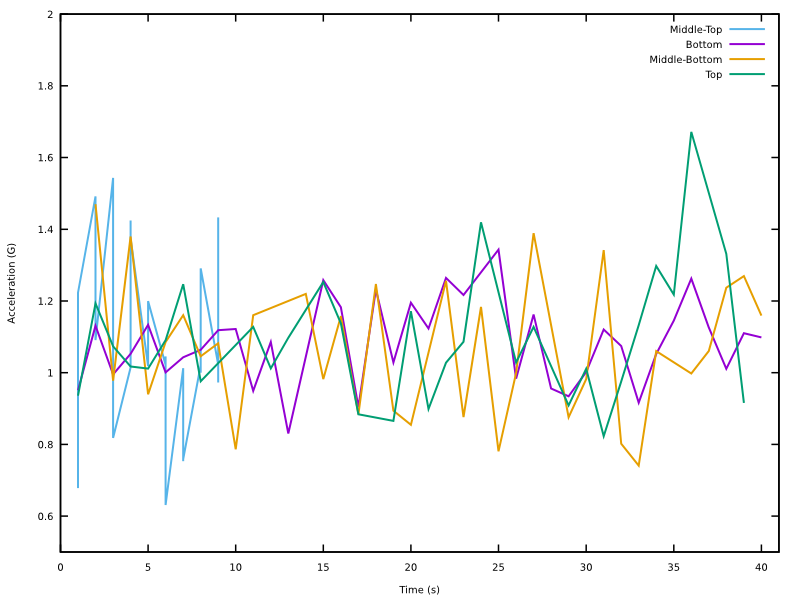
\includegraphics[width=0.5\textwidth]{img/same-level-data}
  \caption{Results for all sensors at the same intensity}
  \label{fig:same-level}
\end{figure}

One final test performed with the sensors on the shake table was to place them in the middle of a shelf, instead of placing them on the side. In theory, if the material is too elastic 
or the structure is not properly built to absorb shocks, its weakest point would be in the very middle. This means that after an intense vibration, the sensors would still be getting 
readings of over 1G even after the source of the vibrations (suppose an earthquake) no longer exists. In figures \ref{fig:middle-4} and \ref{fig:middle-5}, we see the results of this 
experiment as seen at the lowest level (sensor ID 4) and the highest level (sensor ID 5). In the graph, we have kept the sensors on for 40 seconds after shacking the table at different 
intensities. It can be seen that, for sensor 4, we are still getting readings, but they are nothing too significant, being under 1.5G. For sensor 5, we see that the same applies for small 
and, to some extent, medium intensities. However, once we get to high intensity vibrations, due to the elastic nature of the table's material, we are still getting readings that reach 2G.
This shows that we could potentially use these sensors to detect eventual flaws in the structure of buildings.

\begin{figure}[ht] \centering
  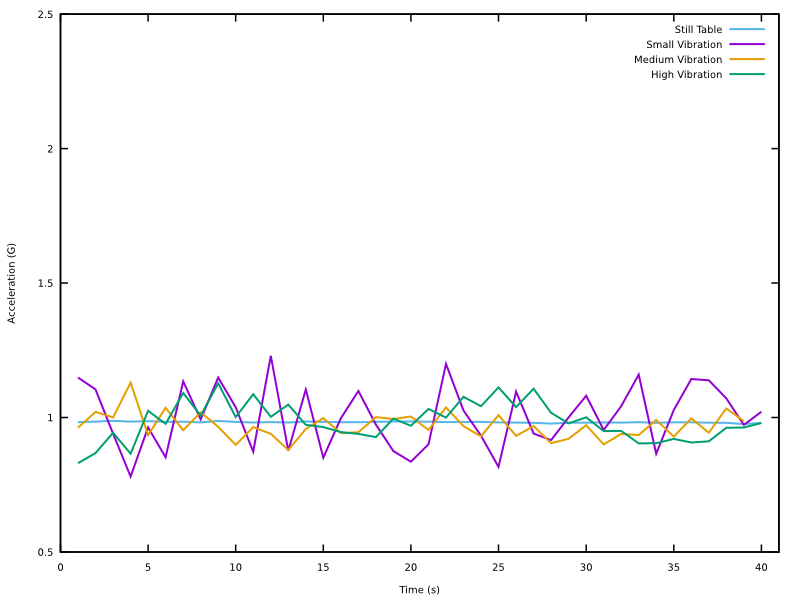
\includegraphics[width=0.5\textwidth]{img/sensor-4-middle}
  \caption{Results for sensors 4 placed in the middle of the shelf}
  \label{fig:middle-4}
\end{figure}

\begin{figure}[ht] \centering
  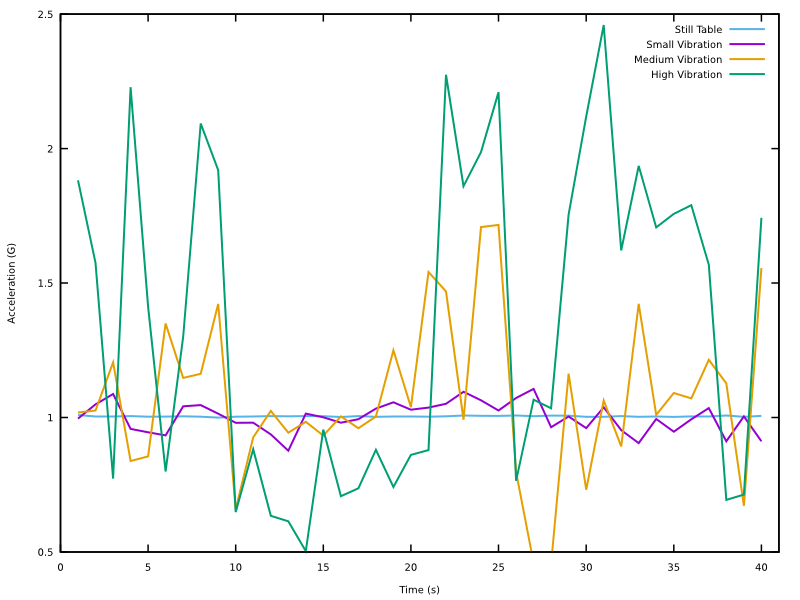
\includegraphics[width=0.5\textwidth]{img/sensor-5-middle}
  \caption{Results for sensors 5 placed in the middle of the shelf}
  \label{fig:middle-5}
\end{figure}

